The future work will be focused on trying to find an answer to the RQ3 during the second part of the research.
In order to achieve it, a detailed study of the current state of the art of features involved with multi-robot choreography such as emergent properties or collaborative strategies must be performed.
Nevertheless, since our plan is to continuously integrate all the obtained knowledge into the research the framework developed during the first division of the project will be used and tested through this part as well.
Furthermore, due to the tools created for the robot orchestration will be tested on real robots we still will need to deploy the software platform and its functionalities on each of them.
An architectural overview of the whole research is depicted in Figure~\ref{fig:overview}.
In this figure the expected final system is represented in a schematic way.
The aforementioned conceptual and temporal division of the research is expressed with dot-lined boxes.
The contents of the box concerning RQ1 comprehend everything since it represents a broad study.
Then, the research concerning RQ2 is more focused.
The box that represents such research contains a robotic team represented by a group of folded boxes that in turn contain the framework intended for each robot.
The communication methodology is also represented in the figure.
Then, the features that we plan to study in order to perform the choreography are also depicted in the space within the RQ3 box.
Note that the contents regarding the RQ2 are embedded into the RQ3.


\begin{figure}[!t]
\begin{center}
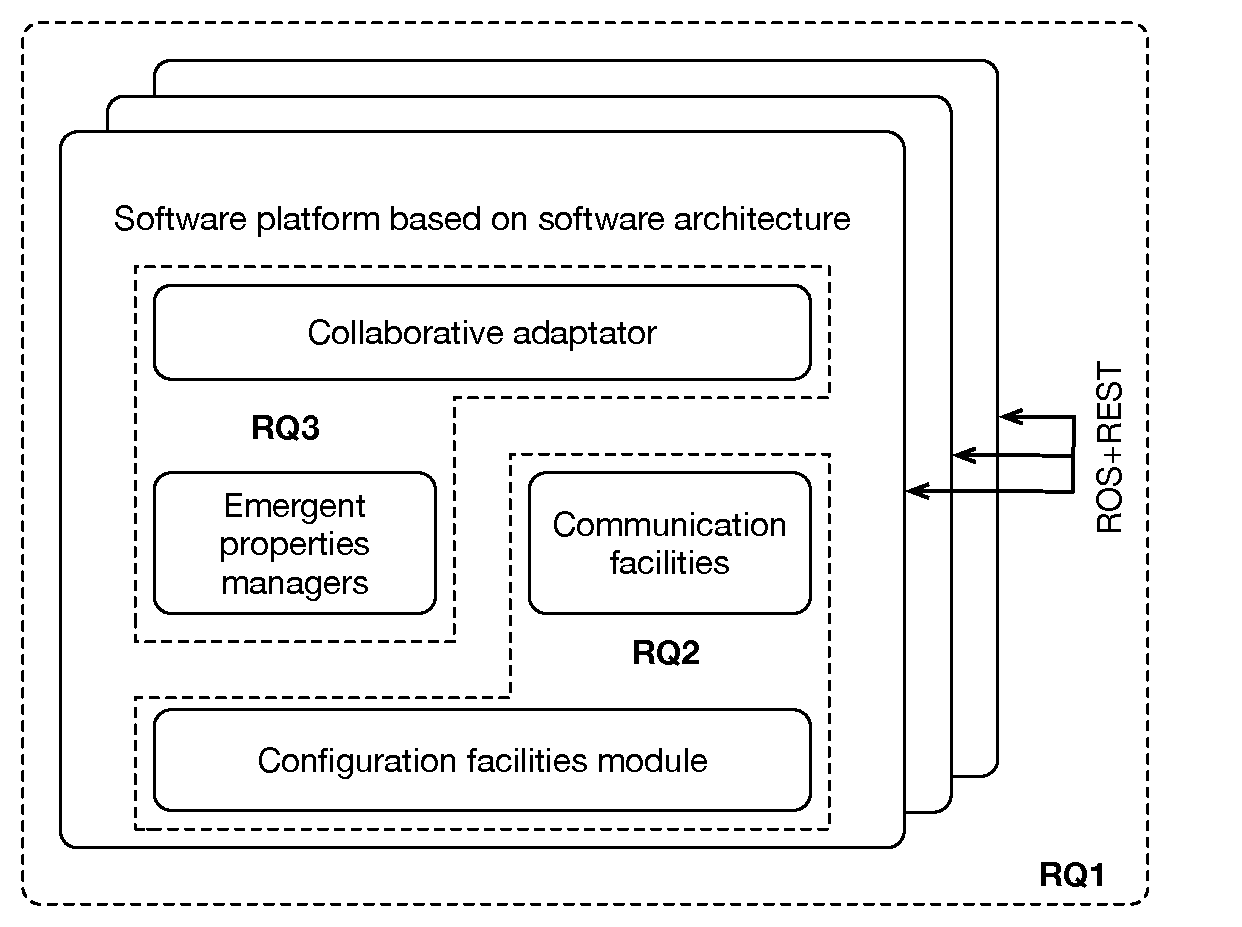
\includegraphics[width=1\linewidth]{Figures/research.pdf}
\caption{Architectural overview of the final system.}
\label{fig:overview}
\end{center}
\end{figure}